\documentclass[twoside]{esi-tfg}

\usepackage{xspace}
\usepackage{blindtext}
\usepackage{custom, tikz, subfigure, float, todonotes, xr, eurosym, longtable, multirow, graphicx, wrapfig, lscape, rotating, color}
\usepackage[table]{xcolor}
\usepackage[export]{adjustbox}

% Control de viudas y huérfanas
\usepackage[defaultlines=4,all]{nowidow}

%Control de espacios en blanco al final del texto (no estirar el texto)
\raggedbottom

% Personalizaciones de estilo
\usetikzlibrary{shapes,shadows}
\tikzstyle{shadowBox} = [draw=black, fill=white, rectangle, inner sep=10pt, style=rounded corners, drop shadow={fill=black,   opacity=1}, text width=14cm]



%% -- Información general --
\title{Memento Parking}
\author{Juan Bausá Arpón}{}


%% -- Variables de la clase esi-tfg --

%- datos del autor

%\address{}
%\city{}
%\country{}
\email{juanbausa@gmail.com}
\phone{}
% \homepage{http://esi.uclm.es/~juan.nadie}


%- datos del documento

%\logo{informatica.pdf}
\advisorFirst{Dr. Manuel Ángel Serrano Martín}
\advisorDepartment{Tecnologías y Sistemas de Información}
%\advisorSecond{Dr. Menganito}
\docdate{2015}{Diciembre}
\intensification{Tecnologías y Sistemas de Información}
%\license{Texto de licencia al gusto de cada uno.}


\begin{document}

\renewcommand\bibname{Bibliografía}

\cover
\bastardtitle
\frontpage

\frontmatter
\copyrightpage
\jury

\chapter{Resumen}

Es un hecho incontestable que actualmente la tecnología sirve como ayuda y apoyo a los más diversos escenarios de nuestra vida. Salir a correr, ir al gimnasio, comunicarnos con las personas de nuestro alrededor, comprar cualquier tipo de artículo, ocupar nuestro ocio, recordarnos eventos... existen un sin fin de ejemplos diarios en los que la tecnología surge para hacer la vida un poco más sencilla, y yendo un poco más allá, existen también ejemplos que nos muestran el grado de dependencia tecnológica actual.\\
Es en este contexto en el que se encuadra esta herramienta, algo tan habitual como no recordar donde se ha aparcado el vehículo o el que varios miembros de una familia utilicen el mismo vehículo y necesiten saber donde está aparcado, es el principal problema que viene a resolver este \ac{TFG}, mediante una herramienta sencilla, simple y fácil de utilizar.\\
Debido a las características intrínsecas de la misma, el público al que va dirigido no tiene especiales conocimientos en las nuevas tecnologías, por lo que se buscará ante todo la claridad en su utilización para facilitar el aprendizaje de personas no acostumbradas al uso de este tipo de herramientas.\\


\chapter{Abstract}

It is an undeniable fact that at the present time, technology serves as both assistance and support to the most diverse situations in our life. Going jogging, visiting the gym, communicating with the people around us, buying/purchasing a range of different items, spending our leisure time, reminding us about different events... There are countless everyday examples where technology appears/arises to make life a little simpler, and going a little further, there are also examples that show us the current level of technological dependence.
It is in this context that this tool fits, something as common as forgetting where you parked the car, or the fact that several family members use the same vehicle and need to know where it is located, is the main problem/issue this dissertation/thesis intends to resolve through a simple and easy-to-use tool. Owing to/because of its intrinsic characteristics, the audience is aimed at/the target audience does not have special knowledge in new technologies, and therefore, first and foremost, clarity in its use will be sought to make learning easier for people not accustomed to the use of this kind of tool.


\chapter{Agradecimientos}

A mis padres, sin vuestro apoyo no hubiera podido tomar esta decisión, gracias por confiar en mí y ayudarme a llegar hasta el final. Sólo lamento no poder teneros a mi lado en este día.


A mis hermanos, unos me habéis apoyado cuando más lo necesitaba, otros me habéis regañado para que no tirase la toalla y algunos siempre estabais al otro lado del teléfono para escucharme. Pero siempre podía contar con vuestro amor incondicional.


Manuel, sin ti no hubiera podido terminar este proyecto, tu pasión por enseñar y aprender me hizo volver a ilusionarme con aquello que tanto disfruto, gracias por recordarme todo esto y acompañarme en el último tramo.

Jose, tantos años juntos me han servido para valorar una amistad como la tuya. Algo extraordinariamente difícil de encontrar. Siempre recordaré nuestros años viviendo juntos.


Gloria, gracias por estar a mi lado. Gracias por tantos cafés. Gracias por tus correcciones. Gracias por tus discusiones. Gracias por tu sinceridad. Gracias.


Blanca, no tengo palabras suficientes con las que agradecerte todas las horas que hemos pasado juntos. Siempre podrás contar conmigo.


Ana, terminemos juntos esta etapa y comencemos juntos la siguiente.
\vspace{1cm}





\begin{verse}
\noindent
¡Oh, capitán! ¡mi capitán! nuestro terrible viaje ha terminado,\newline
el barco ha sobrevivido a todos los escollos,\newline
hemos ganado el premio que anhelábamos,\newline
el puerto está cerca, oigo las campanas, el pueblo entero regocijado,\newline
mientras sus ojos siguen firme la quilla, la audaz y soberbia nave.\newline
Mas, ¡oh corazón!, ¡corazón!, ¡corazón!\newline
¡oh rojas gotas que caen,\newline
allí donde mi capitán yace, frío y muerto!\newline\newline
Walt Whitman
\end{verse}


\quoteauthor{Juan Bausá}

\dedication{A mi padre, in memoriam.}

\tableofcontents
\listoftables
\listoffigures
\lstlistoflistings

\mainmatter

\chapter{Introducción}

\drop{E}{s} evidente que las nuevas tecnologías han cambiado nuestra forma de ver el mundo. No hace más veinte años, durante los primeros años de la década de los 90, era raro ver teléfonos móviles, ya que eran productos considerados elitistas. Al poco tiempo de comenzar la socialización mediante la bajada del precio medio, debido a la bajada del coste y las mejoras en las tecnologías de producción, la posesión de un aparato de telefonía móvil, era la norma. Si bien en un principio únicamente servían para realizar llamadas sin necesidad de estar localizado en un punto fijo anclado a la red teléfonica, poco a poco fueron cambiando los hábitos de consumo para llegar a lo que actualmente podemos observar. Las pequeñas pantallas en blanco y negro, útiles para ver la identidad de la llamada que recibías, poco a poco fueron dando a pantallas capaces de mostrar varias líneas de texto al mismo tiempo, necesario para la creciente demanda de mensajes de texto y para albergar pequeños juegos como el famoso snake de Nokia. La llegada de Apple a este mercado supuso una auténtica revolución, ya que cambió el paradigma del teléfono móvil como elemento comunicativo, para convertirlo en algo más.Una estación de trabajo integral llamada a sustituir agendas de trabajo, relojes, reproductores de música, centralitas...\\

% INTERNET

Internet, puede ser considerado una de las diez tecnologías que más ha cambiado el mundo, y probablemente la que más rápidamente lo ha conseguido. La aparición de las primeras enciclopedias, escritas y editadas con la intención de acercar el conocimiento a las masas, fueron escritas con el propósito de recoger y presentar todo el conocimiento que existía en aquella época. Los enciclopedistas, acorde a las ideas de la ilustración, consideraban que cualquier tipo de mal provenía de la ignorancia, y por tanto la manera de combatir la raíz de los problemas era brindar a las personas la oportunidad de acceder al corpus de conocimientos existente, hasta entonces encerrado en las instituciones académicas y eclesiásticas.

Aunque inicialmente las redes de computadores que finalmente acabarían desembocando en lo que actualmente conocemos como Internet, eran de uso militar, en el año 1983 ARPANET comienza su andadura permitiendo el intercambio masivo de datos masivo con el acceso de universidades y centros de investigación.%http://www.analfatecnicos.net/pregunta.php?id=77

En el año 2012 existían en internet 634 millones de páginas web. La enciclopedia de Diderot y d'Alembert comprendía un total de 28 volúmenes con 72.999 artículos. %https://es.wikipedia.org/wiki/L%27Encyclop%C3%A9die http://aci.info/2013/10/24/the-history-and-evolution-of-the-internet-media-and-news-in-5-infographics/

Pero la cantidad disponible de información no es una cuantificación válida de su calidad. El acceso a la información es extremadamente sencillo, pero también lo es la creación de contenidos. De la misma manera que los grandes proyectos enciclopédicos fueron escritos por grandes científicos, matemáticos, ingenieros y filósofos de la época, actualmente cualquier persona con un ordenador puede crear contenido fácilmente y ponerlo a disposición del mundo.

La geolocalicalización es una faceta omnipresente en la vida diaria actual, es por ello que no resulta extraño que los dispositivos móviles guarden automáticamente la posición en la que se realiza una fotografía o el lugar desde donde se escribe un comentario en una red social.

// TERMINAR ENLAZANDO LOS TRES TEMAS

// PRESENTAR EL PROYECTO
Conociendo este hecho incontrovertible y tomando en cuenta la popularización de los dispositivos de localización geográfica incorporados en la práctica totalidad de los dispositivos móviles del mercado, resulta interesante abordar un trabajo dedicado a ahondar en el conocimiento de temas tan extendidos como la geolocalización, los dispositivos móviles y el desarrollo web.



\begin{figure}[hbtp]
\centering

\subfigure[Árbol de la ciencia de Llull. 1505]{\includegraphics[width=60mm, height=80mm]{./images/Arbol_del_conocimiento.jpg}}
\hspace{10mm}
\subfigure[Portada de L'Encyclopédie. 1751]{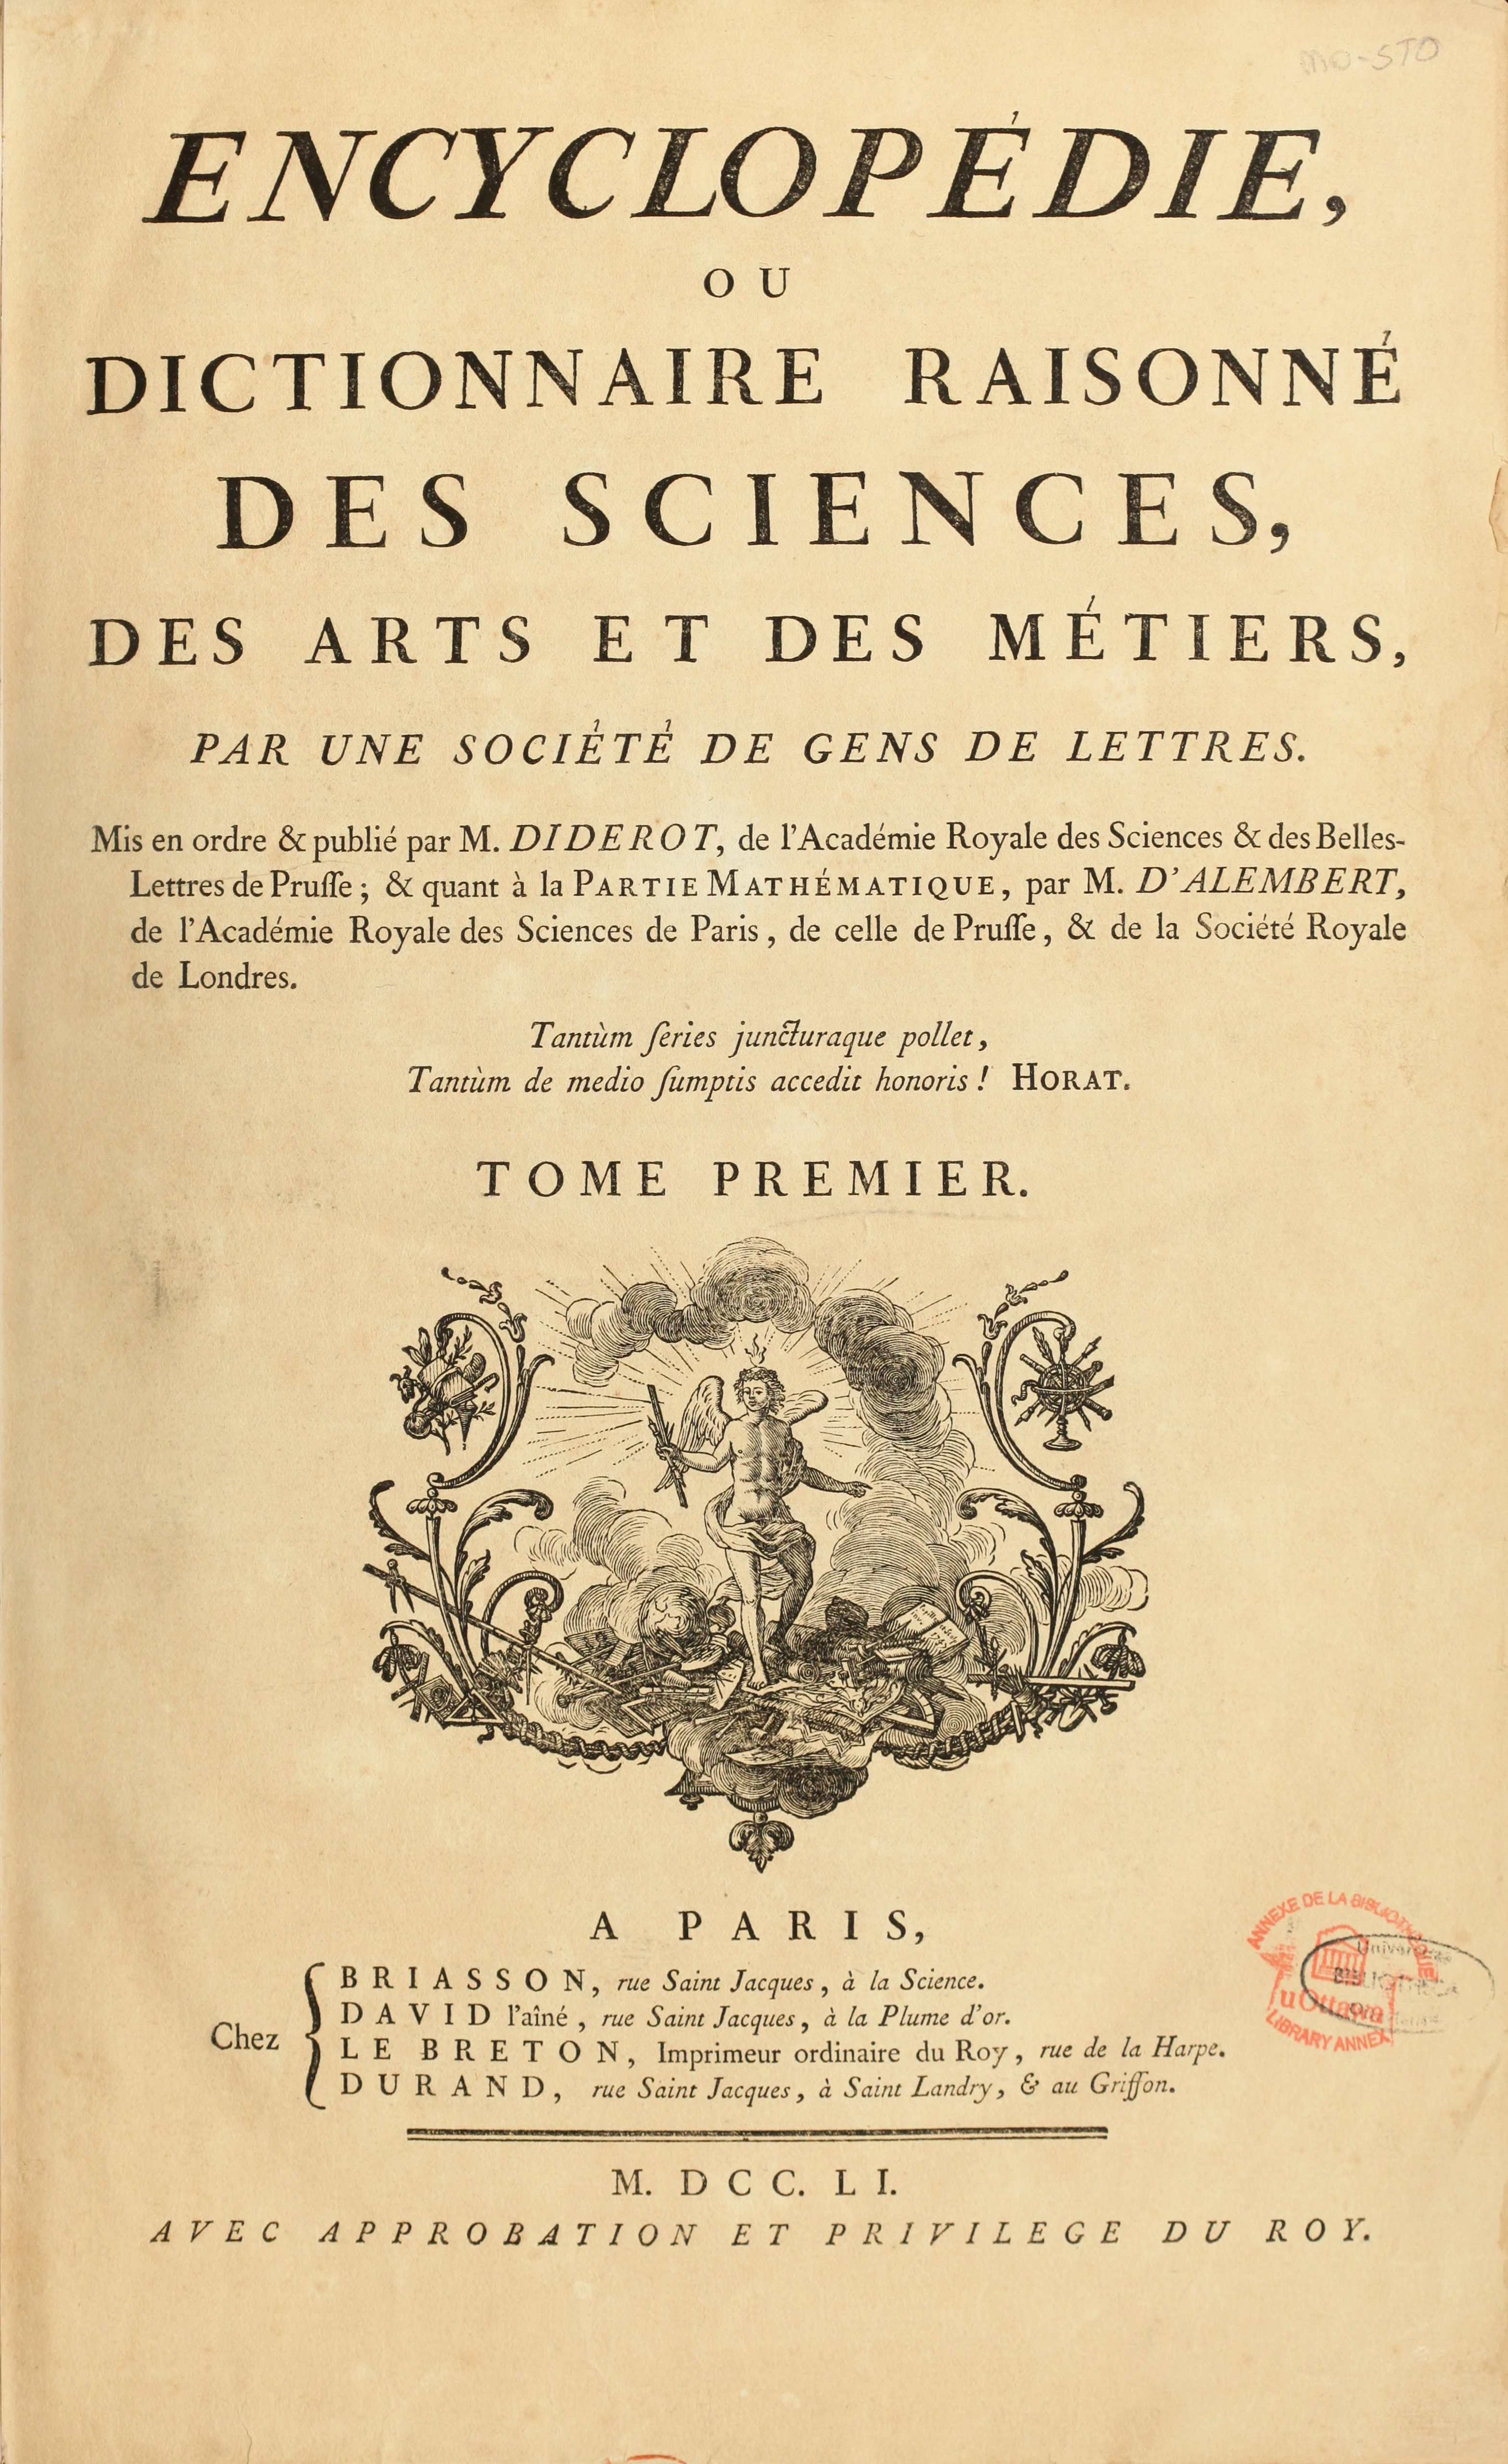
\includegraphics[height=80mm]{./images/Enciclopedia_portada.jpg}}
\vspace{10mm}
\subfigure[Estructura organizada del conocimiento humano. 1752]{\includegraphics[width=80mm, height=110mm]{./images/Conocimiento_humano.jpeg}}

\caption{Árbol de la ciencia de Llull y l'Encyclopédie de Diderot y d'Alembert}\label{fig:Enciclopedia}
\end{figure}

\section{Título del proyecto}

En la portada ---y otras páginas de presentación--- el nombre o título del
proyecto debe aparecer sin comillas, cursiva u otros formatos. Si se cita el
título de otra obra, o el nombre de un capítulo sí debe aparecer entre
comillas. Por cierto, las comillas que deben usarse en castellano son las
«latinas», dejando las ``inglesas'' para los raros casos en los que aparezca una
cita en el cuerpo otra~\cite{sousa}.


\section{Estructura del documento}

Pueden incluirse aquí una sección con algunos consejos para la lectura del
documento dependiendo de la motivación o conocimientos del lector.  También
puede ser útil incluir una lista con el nombre y finalidad de cada uno de los
capítulos restantes.

\begin{definitionlist}
\item[Capítulo \ref{chap:antecedentes}: \nameref{chap:antecedentes}] Explica herramientas
  y aspectos básicos de edición con \LaTeX.
\item[Capítulo \ref{chap:objetivos}: \nameref{chap:objetivos}] Finalidad y justificación
  (con todo detalle) del presente documento.
\end{definitionlist}


\section{Más texto para que ocupe varias páginas}

\blindtext
\blinditemize[4]
\blindmathpaper


% Local Variables:
%  coding: utf-8
%  mode: latex
%  mode: flyspell
%  ispell-local-dictionary: "castellano8"
% End:

\chapter{Objetivos}
\label{chap:objetivos}

\noindent
%Para este capítulo, la normativa indica:
%
%«Concretar y exponer el problema a resolver describiendo el entorno de trabajo,
%la situación y detalladamente qué se pretende obtener. Limitaciones y
%condicionantes a considerar para la resolución del problema (lenguaje de
%construcción, equipo físico, equipo lógico de base y de apoyo, etc.). Si se
%considera necesario, esta sección puede titularse ``Objetivos e hipótesis de
%trabajo''. En este caso, se añadirán las hipótesis de trabajo que el alumno, con
%su TFG, pretende demostrar».

En este capítulo se expone el objetivo principal del TFG, así como los objetivos parciales que se intentarán conseguir con la realización de este trabajo.

\section{Objetivo general}

%El hito final que se pretende lograr, destacando el problema específico que
%resuelve o la funcionalidad que aporta la aplicación o sistema desarrollado.
El objetivo principal de este TFG consiste en el desarrollo de un producto software que permita al usuario almacenar una posición geográfica (típicamente, el lugar de aparcamiento de uno o varios vehículos) y recuperar más tarde esta posición para mostrarla. El usuario podrá utilizar el producto bien desde un navegador web, accediendo a y autenticándose en el servidor, bien a través del dispositivo móvil \ref{fig:Preview_App}. En este último caso, se brinda la opción, una vez recuperada la posición, de mostrar una ruta guiada hasta el lugar de aparcamiento.

%Imagen App (Aproximacion)
\begin{figure}[hbtp]
\centering
\includegraphics[height=60mm, fbox={\fboxrule} 4mm]{images/objetivos/telefono_parking.jpg}
\caption{Aproximación de la aplicación.}
\label{fig:Preview_App}
\end{figure}
%https://dotfirst.io/

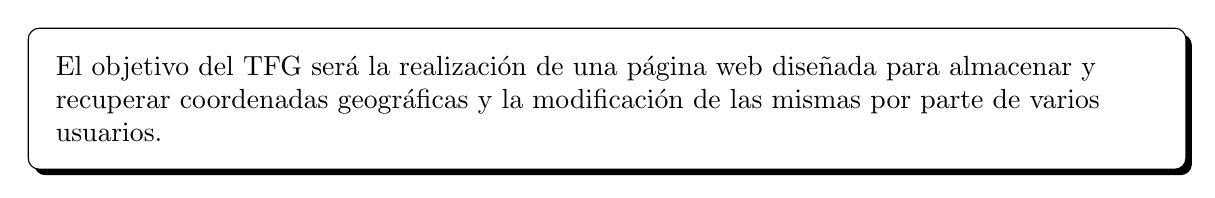
\begin{tikzpicture}
	\node[shadowBox] {El objetivo del TFG será la realización de una página web diseñada para almacenar y recuperar coordenadas geográficas y la modificación de las mismas por parte de varios usuarios.};
\end{tikzpicture}

En la figura \ref{fig:arquitectura} se puede ver un diagrama de la arquitectura del sistema que se implementará en el presente TFG.
\begin{figure}[hbtp]
\centering
\includegraphics[scale=0.75, fbox={\fboxrule} 4mm]{images/objetivos/arquitectura.png}
\caption{Arquitectura de la aplicación}
\label{fig:arquitectura}
\end{figure}


\section{Objetivos específicos}

En la tabla \ref{tab:objetivos}

\begin{table}[hp]
  \centering 
  \rowcolors{1}{gray!25}{white}
  \begin{tabular}{p{0.2\linewidth}p{0.7\linewidth}}
    \multicolumn{1}{l}{\cellcolor{black!30}\textbf{Id Objetivo}} & 
 	\multicolumn{1}{c}{\cellcolor{black!30}\textbf{Descripción del objetivo}}\\
    \toprule
    Objetivo 1 & Realizar una página web para el acceso a la herramienta \\
	Objetivo 2 & Añadir gestión de usuarios a la página (registro y control de acceso) \\
	Objetivo 3 & Permitir el almacenamiento, edición y recuperación de datos a través de la página web \\
	Objetivo 4 & Mostrar los datos almacenados mediante la inclusión de mapa \\
	Objetivo 5 & Facilitar a un usuario permitir a otros usuarios la edición de los datos almacenados \\
	Objetivo 6 & Añadir opción para mostrar recorrido desde el punto actual al punto almacenado \\
    \hline
  \end{tabular}
  \caption{Objetivos parciales del TFG}
  \label{tab:objetivos}
\end{table}


\subsection{Objetivo 1}
\emph{Realizar una página web para el acceso a la herramienta.}\\
El comienzo del desarrollo será la implementación de una página web que sirva como marco y base para el resto de objetivos. Al termino de este punto debe existir una página web accesible con todos los elementos típicos que se un usuario espera encontrar, esto es, una página de inicio, contacto, acerca de, y una estructura reconocible y visualmente agradable. También se prestará atención a la accesibilidad desde dispositivos móviles comprobando que la visualización es correcta y no se pierde ni funcionalidad ni estética al cambiar el método de acceso. En la figura \ref{fig:prototipo_Home} se puede observar un prototipo inicial de la página principal de la aplicación.

% IMAGEN: prototipo_Home
\begin{figure}[hbtp]
\centering
\includegraphics[scale=0.5, fbox={\fboxrule} 4mm]{images/objetivos/prototipo_Home.png}
\caption{Prototipo. Home}
\label{fig:prototipo_Home}
\end{figure}

\subsection{Objetivo 2}

\subsection{Objetivo 3}


% Local Variables:
%  coding: utf-8
%  mode: latex
%  mode: flyspell
%  ispell-local-dictionary: "castellano8"
% End:

\chapter{Antecedentes}
\label{chap:antecedentes}

\drop{E}{n} este capítulo se muestra el trabajo de documentación e investigación previa a la realización del presente \ac{TFG}. En primer lugar se abordarán los sistemas de posicionamiento, su historia y el desarrollo del gps\footnote{Debido al extendido uso de la denominación \textit{GPS} como sinónimo de los \ac{GNSS}, se usará de este modo. Para referirse al sistema de posicionamiento propiedad del gobierno de los Estados Unidos \acf{GPS} se utilizará el acrónimo en mayúsculas} 

y los antecedentes de los \ac{SIG}, más tarde se comentarán algunos aspectos relevantes de la web y de las tecnologías móviles. Para terminar, se enumerarán algunas aplicaciones similares que podemos encontrar actualmente en el mercado.

\section{Localización geográfica y \acf{SIG}}

%HISTORIA DEL GPS
Los \ac{GNSS} permiten conocer en tiempo real la posición de un objeto cualquiera en la superficie terrestre.

Según Scott Gleason y Demoz Gebre-Egziabher \cite{Glea09} podríamos definir la navegación como:

	\vspace{5mm}
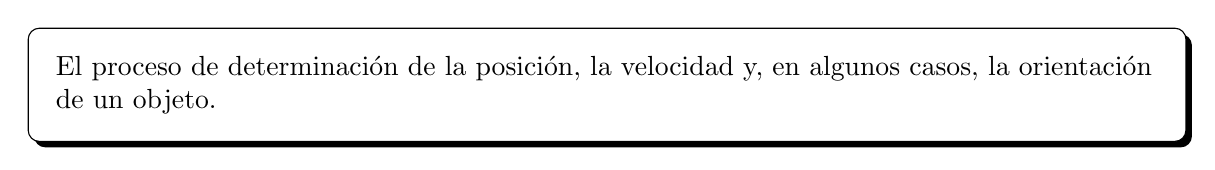
\begin{tikzpicture}
	\node[shadowBox] {El proceso de determinación de la posición, la velocidad y, en algunos casos, la orientación de un objeto.};
\end{tikzpicture}
	\vspace{5mm}

Por tanto, un \ac{GNSS} consiste en una constelación de satélites que permiten determinar con precisión las coordenadas geográficas y la altitud de un punto dado en cualquier punto de la superficie terrestre.

El inicio de este tipo de sistemas podríamos encontrarlo en los primeros marinos. La decisión de alejarse de las rutas que transcurrían a lo largo de la línea de visión de la costa, con la intención de reducir el tiempo, los costes derivados de los viajes y la posibilidad de encontrar nuevos mercados, planteó un nuevo reto tecnológico consistente en conocer con exactitud la localización en la que se encontraban.
La primera solución vino de la mano de un gran conocimiento de la bóveda celeste y la posición de las estrellas. Usando instrumentos como el astrolabio y el sextante (ver figura \ref{fig:sextante_astrolabio}), se podía calcular con asombrosa exactitud la posición.

\begin{figure}[hbtp]
	\begin{adjustbox}{minipage=\linewidth, fbox}
		\centering
		\subfigure[Sextante]{\includegraphics[width=60mm, height=80mm]{./images/03-antecedentes/04-sextante.png}}
		\hspace{10mm}
		\subfigure[Astrolabio]{\includegraphics[height=80mm]{./images/03-antecedentes/05-astrolabio.png}}
	\end{adjustbox}
	\caption{Primeros instrumentos de navegación}
	\label{fig:sextante_astrolabio}
\end{figure}

Hasta tiempos recientes (segunda mitad del S. XX), con la irrupción del posicionamiento satelital, este era el método usado para conocer la ubicación en la que se encontraban.
Los primeros prototipos del gps se desarrollan a principios del S. XX, coincidiendo con los comienzos de la automoción, aspecto este último que ha dado la gran fama a esta tecnología.
El primer gps data de 1909, que consistía en un odómetro que giraba un mapa indicando los hitos más importantes que se podían encontrar en el punto kilométrico en el que estabas.
Este primer prototipo se llamaba \textit{Jones Live Map} (ver figura \ref{fig:jones_live_map}), cada mapa era válido para unos 160 km y después había que cambiarlo por el siguiente mapa. Este primer intento dejó de fabricarse en los años 20, cuando las carreteras estaban correctamente señalizadas \cite{GPS12}.

\begin{figure}[hbtp]
\centering
\includegraphics[scale=0.5, fbox={\fboxrule} 4mm]{images/03-antecedentes/06-jones_live_map.png}
\caption{Jones Live Map}
\label{fig:jones_live_map}
\end{figure}

También en la década de los veinte, hizo su aparición el \textit{Plus Fours Routefinder} (ver figura \ref{fig:plus_fours_routefinder}), consistente en un pequeño reloj de muñeca con una serie de papiros con la información de la ruta que debían ir desenrollándose de forma manual para ir viendo las indicaciones \cite{Plus14}.

\begin{figure}[hbtp]
\centering
\includegraphics[scale=0.5, fbox={\fboxrule} 4mm]{images/03-antecedentes/07-plus_fours_routefinder.png}
\caption{Plus Fours Routefinder}
\label{fig:plus_fours_routefinder}
\end{figure}

Otro de los padres del gps moderno es el llamado \textit{Iter Avto} (ver figura \ref{fig:iter_avto}), consistente en un mapa enrollado conectado al velocímetro del coche para sincronizarlo. La dos grandes ventajas con respecto al \textit{Plus Fours Routefinder}, consistía en que se instalaba sobre el salpicadero del coche y mostraba de forma gráfica la posición. Su inconveniente, cualquier desviación de la ruta era completamente indetectable \cite{Parra13}.

\begin{figure}[hbtp]
\centering
\includegraphics[scale=0.5, fbox={\fboxrule} 4mm]{images/03-antecedentes/08-iter_avto.png}
\caption{Iter Avto}
\label{fig:iter_avto}
\end{figure}

Durante la segunda guerra mundial, la \ac{RAF} desarrolló un sistema de
posicionamiento para sus bombarderos consistente en tres estaciones de radar que localizaban
con precisión al avión \cite{Ori13}.
Los verdaderos orígenes de los gps como sistema de navegación satelital se remontan a 1957 con
el programa \textit{TRANSIT}. Por un lado la marina de los estados unidos inicia el programa \textit{Polaris},
que consiste en el despliegue de misiles transcontinentales suboceánicos. Alcanzar los objetivos
con los misiles dependía de la capacidad de determinar con precisión la posición de los
submarinos en cualquier punto de la superficie terrestre. Por otro lado, la universidad Johns
Hopking de Maryland, consigue determinar con precisión la órbita del \textit{Sputnik 1} a partir del
desplazamiento Doppler sufrido por la señal que emitía y el conocimiento preciso de la posición
del receptor. Con estos elementos, invertir los términos del problema resultó relativamente
sencillo, esto es, conociendo la posición de un satélite de forma precisa, es posible determinar
la de un receptor situado en el submarino de posición desconocida midiendo el desplazamiento
Doppler sufrido por la señal emitida del satélite.

El sistema \textit{TRANSIT} entró en funcionamiento en 1964 con el lanzamiento de 10 satélites y se mantuvo en servicio
hasta 1996. En 1967 se permitió su uso civil. El error típico de este sistema era de unos 250
metros, por lo que resultaba muy útil para la navegación de aviones, barcos y submarinos, pero
por razones obvias (precisión y tamaño de los receptores) aún estaban lejos de los sistemas de
navegación personal actuales.

La Unión Soviética había desarrollado casi al mismo tiempo, un sistema muy parecido con
idénticas prestaciones, el \textit{TSICADA}, lo que resultaba inadmisible para los norteamericanos en el
contexto de la guerra fría, por lo que comenzó a desarrollarse lo que posteriormente sería el
\ac{GPS} \cite{Pala10}.
El \textit{NAVSTAR-GPS} nació en 1973 para uso exclusivamente militar, con una constelación de 24
satélites en órbitas inclinadas de 12 horas, lo que se traducía en que cualquier receptor en el
mundo tendría en su horizonte visible al menos 5 satélites disponibles en todo momento. El
TRANSIT, no sólo no podía garantizar esto, debido a que sus satélites eran de órbita baja, si no
que con sus 6 satélites, algunos receptores podían estar varias horas esperando señal. El primer
satélite se puso en órbita en 1978. La precisión de este nuevo sistema era de 1 metro y podía
ser incorporado en misiles, bombas inteligentes, vehículos, etc. Debido a su consideración de
recurso de gran valor estratégico, su uso estaba limitado al ámbito estrictamente militar.
El 31 de agosto de 1983 tuvo lugar uno de los incidentes internacionales más graves de la
guerra fría, que a la postre resultaría decisivo para el uso actual del \ac{GPS}, el derribo del vuelo de
\textit{Korean Airlines KAL007} por parte de la \ac{URSS} \cite{Kore15}.

El citado vuelo, usando los sistemas de navegación tradicionales disponibles en aquella época, y
usando el piloto automático, invadió en dos ocasiones el espacio aéreo de la Unión Soviética,
que acabó interceptándolo mediante dos cazas militares y derribándole con un ataque con
misiles, matando al pasaje y la tripulación completa, con un resultado de 269 fallecidos.
La respuesta internacional no se hizo esperar, y el entonces presidente de \ac{USA}, Ronald Reagan,
anunció que el sistema \ac{GPS} estaría disponible para propósitos civiles una vez finalizase el
proyecto, con la intención de que no se volvieran a repetir incidentes similares.
Para evitar que sus enemigos pudieran hacer uso de esta nueva tecnología para construir
misiles de precisión con los que atacarlos, el Departamento de Defensa de \ac{EE.UU.} impuso una
serie de restricciones en la precisión de los receptores, de manera que el error en el
posicionamiento fuera mayor que el de los disponibles para uso militar. Por ello los receptores de gps de uso
civil eran incapaces de mostrar una resolución menor de 20 metros.
Durante la primera guerra del golfo, en 1991, se desarrolló una mejora en la precisión del \ac{GPS}
llamada, \ac{GPS} Diferencial, que conseguía precisiones de entre 1 y 3 metros de exactitud.

\subsection{Funcionamiento de los gps}

La base sobre la que se asienta el funcionamiento del posicionamiento mediante satélites consiste en que sea cual sea nuestra localización en la corteza terrestre, siempre estaremos a la vista de al menos cuatro satélites distintos.

Cada uno de estos satélites transmite información acerca de su localización que será utilizarada por nuestro receptor para calcular la distancia a la que se encuentran, en función del tiempo que tardan las señales en llegar.
Conociendo la distancia a la que se encuentran, como mínimo, tres satélites, es posible conocer con un cierto grado de aproximación la zona en la cual debemos estar posicionados. Este proceso de localizacion se conoce como triangulación.

Si estamos al alcance de un único satélite, la posible zona en la que nos encontraremos será todo el área de influencia del mismo. En el caso de utilizar dos satélites, la zona en la que podríamos encontrarnos sería la superficie de la intersección de las dos esferas imaginarias creadas con centro cada uno de los satélites y radio la distancia a nuestra posición.

En el caso de utilizar tres satélites, que como hemos comentado anteriormente es el mínimo necesario, la posible localización se ve reducida a dos puntos. Para conocer con precisión cual de esos dos puntos es el correcto haría falta un cuarto satélite, pero en términos generales, uno de ellos no estará ubicado en la corteza terrestre, por lo que podrá descartase y conocer de esta manera nuestra localización (ver figura \ref{fig:triangulacion-satelital}).

\begin{figure}[h!btp]
\centering
\includegraphics[scale=0.5, fbox={\fboxrule} 0mm]{images/03-antecedentes/31-funcionamiento_gps.jpg}
\caption{Triangulacion satelital}
\label{fig:triangulacion-satelital}
\end{figure}

Debido a razones de obvias de estrategia militar, la precisión dada por los satélites \ac{GPS} incluía un cierto grado de error aleatorio llamado \textit{disponibilidad selectiva}. Este error fue eliminado el 2 de mayo del año 2000. Habitualmente la precisión para usos civiles se veía limitada a 100 metros \cite{Corr00}.

\subsection{Cartografía\footnote{La labor de documentación está basada en: \cite{Diaz15}.} y \acs{SIG}}

Antes de la aparición de la historia, esto es, antes de la constatación escrita de los acontecimientos, se produjo la aparición de los mapas. Estos estaban realizados con la intención de establecer distancias, recorridos y localizaciones de elementos de cierta importacia.

El mapa más antiguo del que se tiene noticia proviene de la antigua Babilonia y está fechado alrededor de 4500 años a.C. Actualmente está conservado en Museo Británico (ver figura \ref{fig:mapa-babilonio}).

\begin{figure}[h!btp]
\centering
\includegraphics[scale=0.5, fbox={\fboxrule} 0mm]{images/03-antecedentes/32-mapa_babilonio.jpg}
\caption{Tablilla babilónica y reconstrucción}
\label{fig:mapa-babilonio}
\end{figure}

La antigua Grecia fue quien colocó las bases para la cartografía actual, aportando grandes conocimientos geométricos, matemático geográficos y  astronómicos. Los cartógrafos griegos, que admitían la forma esférica de la tierra, fueron los iniciadores del sistema de localización geográfica, es decir, las latitudes y longitudes, hicieron las primeras proyecciones \cite{Schl07} y dieron una cifra bastante aproximada del tamaño de nuestro planeta \cite{Aup09}.

Prácticamente todo lo que conocemos de la cartografía de este tiempo se debe a los escritos de Herodoto y Estrabón que mencionan a Anaximándro de Mileto como el realizador de un mapa completo de la tierra incorporando mares y ríos \cite{Kap10}. Pero de entre todos los personajes de la antigua gracia, fue Claudio Ptolomeo el más importante para el campo de la cartografía con su obra \textit{Geographia} en la que se puede apreciar un mapamundo que abarca desde las islas Canarias por el oeste hasta China por el este (ver figura \ref{fig:mapa-ptolomeo}). Debido a que en este mapa aparecen las latitudes, el ecuador la escala y está orientado al norte, es posible apreciar las bases de las cartas de navegación modernas.

\begin{figure}[h!btp]
\centering
\includegraphics[scale=0.5, fbox={\fboxrule} 0mm]{images/03-antecedentes/33-mapa_ptolomeo.jpg}
\caption{Mapa Ptolemáico}
\label{fig:mapa-ptolomeo}
\end{figure}

Durante la era romana se sufrió un retroceso en la cartografía, que no volvería a los niveles griegos hasta el siglo XVI, ya que estaban más interesados en la realización de mapas prácticos de fines militares, administrativos y comerciales que en plasmar la realidad sobre el papel.

Durante la edad media, se pierde el concepto de esfera en los mapas y se representa el mundo ateniéndose más a conceptos místicos y religiosos que a la propia realidad. Normalmente aparece Jerusalén en el centro del mapa, como ejemplo en la figura \ref{fig:mapa-beato-liebana} se puede observar el mapamundi incluido de Beato de Liébana.

\begin{figure}[h!btp]
\centering
\includegraphics[scale=0.5, fbox={\fboxrule} 0mm]{images/03-antecedentes/34-mapa_beato_liebana.jpg}
\caption{Mapamundi de Beato de Liébana}
\label{fig:mapa-beato-liebana}
\end{figure}

En el año 1154, Al Idrisi, cartógrafo ceutí, presenta un mapa alejado de las convenciones europeas existentes en la época y más cercanos a los planteamientos griegos. En su mapa se puede observar con gran detalle los perfiles de Europa, norte de Africa y gran parte de Asia, aunque está orientado hacia el sur, en lugar de la orientación norte a la que estamos acostumbrados (ver figura \ref{fig:mapa-al-idrisi}).

\begin{figure}[h!btp]
\centering
\includegraphics[scale=0.5, fbox={\fboxrule} 0mm]{images/03-antecedentes/35-mapa_al_idrisi.jpg}
\caption{Mapamundi de Abu Abd Allah Muhammad al-Idrisi.1154}
\label{fig:mapa-al-idrisi}
\end{figure}

A mediados del siglo XV da comienzo la cartografía moderna como consecuencia de la recuperación de los escritos de Ptolomeo, la invención de la imprenta y la posibilidad de divulgar los mapas con facilidad y los grandes avances técnicos respecto a la brújula y las embarcaciones, que permitían hacer viajes más largos, para lo que necesitaban mejores cartas de navegación.

En el año 1500 aparece el mapa de Juan de la Cosa, y aunque no existe consenso al respecto, la mayor parte de los autores consideran que este es el primer mapa en que aparece América \cite{Verl06}, aunque hay que esperar al año 1507 para poder ver el nuevo continente con su nombre, propuesto por Américo Vespucio, en el mapa de Martin Waldseemüller (ver figura \ref{fig:mapas-america}).

\begin{figure}[h!btp]
	\begin{adjustbox}{minipage=\linewidth, fbox}
		\centering
		\subfigure[Mapamundi de Juan de la Cosa. 1500]{\includegraphics[width=60mm, height=80mm]{./images/03-antecedentes/36-mapa_juan_de_la_cosa.jpg}}
		\hspace{10mm}
		\subfigure[Mapamundi de Martin Waldseemüller. 1507]{\includegraphics[height=80mm]{./images/03-antecedentes/37-mapa_martin_waldseemüller.jpg}}
	\end{adjustbox}
	\caption{Primeros mapas de América}
	\label{fig:mapas-america}
\end{figure}

Ya en el siglo XX, el desarrollo de la fotografía y la aviación, en el contexto de la Gran Guerra y sobre todo durante la Segunda Guerra Mundial, permitió una gran revolución cartográfica. Siendo conscientes de la gran ventaja militar que suponía el profundo conocimiento del terreno, empiezan a desarrollarse grandes proyectos en este sentido, que culminarán durante la segunda mitad del siglo, en la cartografia de precisión mediante satélites \cite{Lind06}.

Debido a que el término \ac{SIG} engloba la integración de muy diversas áreas,no existe una única definición totalmente consensuada \cite{Chr97}. La definición aportada por el \ac{NCGIA} resulta ampliamente aceptada:

\vspace{5mm}
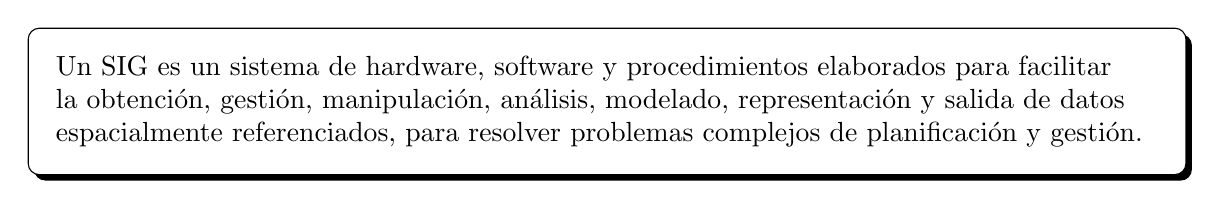
\begin{tikzpicture}
	\node[shadowBox] {
	Un SIG es un sistema de hardware, software y procedimientos elaborados para facilitar la obtención, gestión, manipulación, análisis, modelado, representación y salida de datos espacialmente referenciados, para resolver problemas complejos de planificación y gestión.};
\end{tikzpicture}
\vspace{5mm}

Uno de los elementos relevantes de los \ac{SIG} son la asociación de información a una imagen concreta y una de las primeras muestras de esto lo podemos encontrar en el Londres victoriano de mediados del siglo XIX. En el año 1854, el doctor John Snow (ver figura \ref{fig:john_snow}) utilizó un mapa del Soho londinense para ubicar los casos de un brote de cólera (ver figura \ref{fig:cholera_map}). Con la ayuda de los registros del hospital de Middlesex y de Henry Whitehead, párroco local, recogió las defunciones producidas mediante una fina línea de color negro que se apilaban unas sobre otras a medida que se producían las muertes, consiguiendo el efecto de asociación de información a imagen comentado en el párrafo anterior \cite{Cai11}.

Este ejemplo temprano, combinado con la geolocalización nos permite identificar las líneas base de representación de lo que será el presente \ac{TFG}.

\begin{figure}[hbtp]
\centering
\includegraphics[scale=1, fbox={\fboxrule} 0mm]{images/03-antecedentes/02-john_snow.jpg}
\caption{Doctor Sir John Snow}
\label{fig:john_snow}
\end{figure}

\begin{figure}[hbtp]
\centering
\includegraphics[scale=0.5, fbox={\fboxrule} 4mm]{images/03-antecedentes/01-cholera_map.jpg}
\caption{Mapa del Soho con los casos de fallecimiento por cólera}
\label{fig:cholera_map}
\end{figure}

Gracias a ello y referenciando en el mapa la posición de los pozos de agua, pudo comprobar como una gran cantidad de víctimas se encontraban dentro de la zona de influencia de una bomba de agua en Broad Street (ver figura \ref{fig:cholera_map_detail}), que a la postre resultó estar contaminada con heces. Recomendando la clausura de la misma consiguió acabar con la epidemia      \cite{Gunn07}. Debido a estos logros se le considera el padre de la epidemiología moderna y podemos ilustrar uno de los primeros ejemplos del uso de los \ac{SIG}.

\begin{figure}[hbtp]
\centering
\includegraphics[scale=0.5, fbox={\fboxrule} 4mm]{images/03-antecedentes/03-cholera_map_detail.png}
\caption{Detalle del mapa del Doctor Snow}
\label{fig:cholera_map_detail}
\end{figure}

\section{Internet y la \ac{www}}

%Historia de Internet
Internet puede considerarse como una de las tecnologías que más ha cambiado el mundo y la que más rápidamente lo ha hecho. Gracias a este nuevo concepto, se puede acceder rápidamente a la mayor cantidad de información nunca antes recopilada en la historia de la humanidad.\\

La gran biblioteca de Alejandría, la mayor de las bibliotecas del mundo antiguo, contenía, según Flavio Josefo, antes de su destrucción unos 200.000 volúmenes y consideraban que todo el conocimiento de la humanidad ocuparía un total de 500.000 volúmenes  \cite{Jos94}. Autores modernos han recalculado el posible número de volúmenes, aportando una cifra de unos 50.000 rollos, que podría equivaler a unos 12.500 libros actuales \cite{Esco01}.\\

Los Archivos Secretos Vaticanos contienen un total de 1.600.000 volúmenes \cite{Bav15}, la biblioteca nacional de España 28 millones \cite{Sanz15} y la biblioteca del congreso de los \ac{EE.UU.} 160 millones de documentos \cite{Libr15}. Comparando las cifras de algunas de las mayores bibliotecas del mundo con el número de documentos existentes en Internet, podemos hacernos una idea de lo que esta tecnología a supuesto para la humanidad, no solamente en el volumen de información existente, si no en la facilidad de acceso a los mismos. En el año 2012, en Internet existían un total de 8.310 millones de documentos accesibles.

Aunque no es lícito comparar estas cifras en bruto, ya que tal la cantidad no siempre está relacionada con la calidad, como dijo el escritor Neil Gaiman \cite{Gaim10}:

\vspace{5mm}
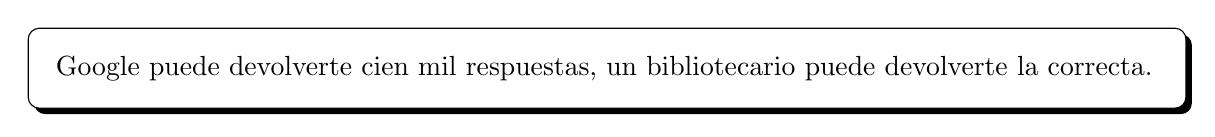
\begin{tikzpicture}
	\node[shadowBox] {
	Google puede devolverte cien mil respuestas, un bibliotecario puede devolverte la correcta.};
\end{tikzpicture}
\vspace{5mm}

En el año 1958 la compañía Bell crea el primer módem, un dispositivo capaz de transmitir datos binarios utilizando una línea telefónica (ver figura \ref{fig:bell_modem}). En el año 1962 J.C.R Licklider describe su concepto de \textit{Red galáctica}, consistente en una red interconectada globalmente que permitiera acceder a todo tipo de datos y programas desde cualquier sitio. Un año antes, en 1961, Leonard Kleinrock publicó su tesis doctoral acerca de la teoría de colas, que sería publicado como libro en el año 1964 (\cite{Klei64}) y que sirvió de fundamento a la teoría de conmutación de paquetes. Los datos se troceaban en partes, llamadas \textit{paquetes}, a los que se les asignaba un número de secuencia antes de enviarlos. De esta manera, no importaba en orden en que llegasen al receptor, puesto que podría recomponer el mensaje original.
En el año 1967 en una conferencia, se presentaba el proyecto inicial de \ac{ARPANET}. Durante las discusiones iniciales del proyecto se llegó a la conclusión de desligar la comunicación de la máquina principal, crean pequeños computadores que fuesen quienes cargasen con la responsabilidad de lidiar con las líneas telefónicas. El 29 de Octubre de 1969 se transmite el primer mensaje a través de \ac{ARPANET} y el 21 de Noviembre de ese mismo año se establece la primera conexión entre las computadoras de la universidad de Stanford y \ac{UCLA}. 

\begin{figure}[hbtp]
\centering
\includegraphics[scale=0.5, fbox={\fboxrule} 4mm]{images/03-antecedentes/09-modem_bell.jpg}
\caption{Módem Bell. 1958}
\label{fig:bell_modem}
\end{figure}

En el año 1972 al calor de una grande y exitosa demostración de \ac{ARPANET}, se introduce la primera gran aplicación de esta nueva tecnología, el correo electrónico. Ray Tomlinson, había desarrollado para \ac{ARPANET} unos años antes un programa llamado SNDMSG para enviar mensajes entre las distintas terminales de una computadora, por lo que adaptó este programa para permitir el envío dentro de una red más amplia.

Con el crecimiento de la red, se desarrollaron tres protocolos que actualmente siguen en uso, \ac{TCP}, \ac{IP} y \ac{DNS}. El año 1983, \ac{ARPANET} se abre definitivamente a la vida civil permitiendo el intercambio masivo de datos entre universidades y centros de investigación. Este es el motivo último por el que se celebra ese año como el nacimiento de Internet.

La \textit{web} (\ac{www}) es probablemente el punto más visible de Internet. Fue desarrollado entre 1989 y 1990 por Tim Berners-Lee y Robert Cailiau mientras trabajaban en el \ac{CERN}.

En la web, es utilizado \ac{HTTP} como protocolo de comunicación, que define la sintaxis y la semántica necesarias para el correcto funcionamiento de los distintos componentes de la comunicación web, consiguiendo una abstracción que permite unificar la forma de comunicación en la red. En las comunicaciones en red el modelo de arquitectura más extendido es el paradigma Cliente - Servidor (ver figura \ref{fig:cliente-servidor}), mediante el cual se define una máquina \textit{servidor} encargada de generar la corriente datos y una serie de máquinas conocidas como \textit{clientes}, que realizan peticiones para consumir estos datos. El funcionamiento básico de este modelo podría verse como una farmacia abierta 24 horas (servidor), que está permanentemente a la espera de que alguna persona decida entrar a comprar algún medicamento, momento en el cual busca la droga pedida y se la facilita.

\begin{figure}[hbtp]
\centering
\includegraphics[scale=0.5, fbox={\fboxrule} 4mm]{images/03-antecedentes/10-client_server.png}
\caption{Modelo cliente-servidor}
\label{fig:cliente-servidor}
\end{figure}

Para que estas transacciones puedan darse, los computadores deben poder conocer como comunicarse, lo que en este caso se logra mediante las direcciones\ac{IP}, una serie de 32 bits que designan unívocamente un elemento de una red, y unos pocos pasos intermedios, y transparentes, para el usuario. El cliente, normalmente mediante un navegador web, es decir, mediante un programa creado específicamente para la navegación y visualización de páginas web, introduce el nombre de la página web con la que quiere comunicarse. Este nombre, por ejemplo, \textit{www.usipv6.com}, es enviado automáticamente a unos servidores llamados \ac{DNS}, que son capaces de buscar la dirección \ac{IP} asociada al nombre de la página tecleada y devolver su dirección \ac{IP}, que en este caso podría ser \textit{123.45.67.89} (ver figura \ref{fig:dns-server}). Es fácil ver el porque se utiliza este paso intermedio, debido a que al usuario le resultará mucho más sencillo recordar una página web que una serie de números. Una vez realizada la traducción, el computador se comunica con el servidor a través de la dirección \ac{IP} obtenida y este le responde enviándole la información solicitada.

\begin{figure}[hbtp]
\centering
\includegraphics[scale=0.5, fbox={\fboxrule} 4mm]{images/03-antecedentes/11-dns_server.png}
\caption{Comunicación con servidor DNS}
\label{fig:dns-server}
\end{figure}

Aunque en sus orígenes,la web se desarrolló para transmitir únicamente texto, actualmente, como es fácil ver, se permite la emisión de todo tipo de contenidos multimedia, como audio, vídeo o imágenes. La tarea del cliente, consiste en recibir los datos enviados por el emisor y reinterpretarlos y mostrarlos de manera coherente para el usuario.

Todo esto nos lleva a poder diferenciar claramente dos trabajos distintos dentro de la comunicación web, el trabajo llevado a cabo por el cliente y el trabajo llevado a cabo por el servidor. Para poder desarrollar cada una de estas tareas, existen una serie de tecnologías específicas para el lado del cliente y para el lado del servidor.

\subsection{Tecnologías del lado del servidor}
Como se ha explicado en la sección anterior, el servidor es el encargado de atender las peticiones que los clientes le envían y responderlas adecuadamente. 
En los comienzos de la web los servidores eran meras estaciones de \textit{almacenaje}, que devolvía al cliente peticionario una página web estática (ver figura \ref{fig:static-server}) mientras que en la actualidad, los servidores son capaces de generar el contenido a enviar de forma dinámica (ver figura \ref{fig:dynamic-server}).

\begin{figure}[hbtp]
\centering
\includegraphics[scale=0.5, fbox={\fboxrule} 4mm]{images/03-antecedentes/12-html_request.png}
\caption{Petición a servidor estático}
\label{fig:static-server}
\end{figure}

\begin{figure}[hbtp]
\centering
\includegraphics[scale=0.5, fbox={\fboxrule} 4mm]{images/03-antecedentes/13-html_dynamic_request.png}
\caption{Petición a servidor dinámico}
\label{fig:dynamic-server}
\end{figure}

Algunas de las tecnologías más utilizadas en el lado del cliente son Apache, PHP y MySQL.

Apache es un software que permite a un computador realizar un comportamiento de servidor, esto es, atender a las peticiones de los clientes, ofrecerles servicios y enviarles la información pedida. Esta desarrollado en C y es de código abierto \cite{Apac15}.

PHP es uno de los lenguaje de programación del lado del servidor más extendido y fue uno de los primeros en poder ser incorporado directamente en el código \ac{HTTP}. Fue creado por Rasmus Lerdorf en 1994 y actualmente se encuentra en su versión 5.6.14 \cite{Hist15}.

MySql es un sistema de gestión de bases de datos relacionales desarrollado por MySQL AB (actualmente parte de Sun Microsystems) en 1995 por Michael Widenius, David Axmark and Allan Larsson \cite{Data14}.

\begin{figure}[hbtp]
	\begin{adjustbox}{minipage=\linewidth, fbox}
		\centering
		\subfigure[MySQL]{\includegraphics[scale=0.5]{./images/03-antecedentes/14-mysql.png}}
		\hspace{10mm}
		\subfigure[PHP]{\includegraphics[scale=0.5]{./images/03-antecedentes/15-php.png}}
		\vspace{10mm}
		\subfigure[Apache]{\includegraphics[scale=0.5]{./images/03-antecedentes/16-apache.png}}
	\end{adjustbox}
	\caption{Tecnologías utilizadas en servidores}
	\label{fig:mysql_php_apache}
\end{figure}

\subsection{Tecnologías del lado del cliente}
Dejando de lado la necesidad de contar con un navegador web que permita mostrar e interactuar con las páginas web mostradas, el cliente debe interpretar los datos recibidos por el servidor de manera que pueda traducirlos convirtiéndolos en el concepto de \textit{página web} que conocemos. Tres de los lenguajes más utilizados en este intercambio de datos son \ac{HTML}, \ac{CSS}, JavaScript y \ac{AJAX}.

\ac{HTML} es un lenguaje de marcado que se utiliza para la representación visual de una página web. Está considerado el lenguaje de programación más importante y está a cargo de la W3C \cite{Worl15}. Aunque permite dar formato al texto, actualmente esto suele ser responsabilidad de las hojas \ac{CSS}.

La última versión, \ac{HTML}5, publicada en octubre de 2014 \cite{Adam14} incorpora novedades como etiquetas con codecs, para manejar grandes conjuntos de datos o mejoras en los formularios.

\ac{CSS} es usado para definir el formato de una página web escrita en \ac{HTML}.

\begin{lstlisting}[
  float=ht,
  language = HTML,
  caption  = {«Hola mundo» en HTML y CSS},
  label    = code:hello]
	<!DOCTYPE html>
	<html>
	<head>
	    <title>Hola Mundo en HTML</title>
		<style>
		body {background-color:lightgrey}
		h1   {color:blue}
		p    {color:green}
		</style>
	</head>
	<body>
		<h1>Hola Mundo</h1>
		<p>Mi primera web en HTML y CSS.</p>
	</body>
	</html>
\end{lstlisting}

Javascript es un lenguaje interpretado orientado a objetos implementado normalmente como parte del navegador web.
\ac{AJAX} es utilizado para poder realizar peticiones a un servidor modificando partes concretas de una página, eliminando de esta forma la necesidad de recargar la página completa.

% Desarrollo web (frameworks)


\section{Dispositivos móviles}
Lo teléfonos móviles han cambiado nuestra manera de relacionarnos tanto con el mundo como entre las personas. No hace más de diez años era imposible pensar en poder acceder a Internet desde cualquier lugar o tener la posibilidad de enviar mensajes a través de 
las aplicaciones de mensajería instantánea. Hace veinte o treinta años nadie imaginaba que los teléfonos móviles serían un elemento imprescindible y omnipresente de nuestras vidas ya que en aquella época era símbolo de estatus y gran lujo.

Podríamos comenzar a explicar los intentos de comunicarse a través de grandes distancias con el telégrafo, primer gran antecedente del teléfono, y es que este invento fue algo revolucionario cuando se presentó. Por primera vez se podían comunicar dos puntos distantes de manera instantánea.

Los orígenes del telégrafo se remontan al S. XVIII cuando Claude Chappe desarrolló para el ejército Francés su precursor inmediato, el telégrafo óptico. Este invento consistía en un sistema de comunicación que emitía una señal visual que podía repetirse en la distancia, aunque solo tenía utilidad en las distancias a las que el ojo pudiera abarcar (ver figura \ref{fig:telegrafo_optico}) \cite{Holz94}.

\begin{figure}[hbtp]
	\begin{adjustbox}{minipage=\linewidth, fbox}
		\centering
		\subfigure[Telégrafo óptico de Claude Chappe]{\includegraphics[height=80mm]{./images/03-antecedentes/17-telegrafo_optico.jpg}}
		\hspace{10mm}
		\subfigure[Claude Chappe]{\includegraphics[height=80mm]{./images/03-antecedentes/18-claude_chappe.jpg}}
	\end{adjustbox}
\caption{Telégrafo óptico}
	\label{fig:telegrafo_optico}
\end{figure}

Con la intención de mejorar el alcance de la comunicación y aprovechando los estudios de electromagnetismo de Michael Faraday y las innovaciones de William Sturgeon y Joseph Henry sobre el electroimán, Samuel Morse (ver figura \ref{fig:telegrafo}) ideó una manera de enviar señales entre dos puntos aprovechando las corrientes eléctricas. En un primer momento, el telégrafo consistía en un péndulo que ante la existencia de corriente movía un lápiz que dibujaba de esa manera una línea sobre un papel. Mejorando el prototipo se llego a inventar el famoso código morse, que consta de los consabidos dos elementos: el punto y la raya.

\begin{figure}[hbtp]
	\begin{adjustbox}{minipage=\linewidth, fbox}
		\centering
		\subfigure[Samuel Morse]{\includegraphics[height=80mm]{./images/03-antecedentes/20-samuel_morse.jpg}}
		\hspace{10mm}
		\subfigure[Código morse]{\includegraphics[height=80mm]{./images/03-antecedentes/21-codigo_morse.jpg}}
	\end{adjustbox}
\caption{Telégrafo}
	\label{fig:telegrafo}
\end{figure}

En 1837 Samuel Morse hizo la primera demostración pública del telégrafo en un áula de la universidad de Nueva York. La gran aportación de Morse.

El 24 de mayo de 1844, se terminó la línea que unía Baltimore y Washington, enviando un mensaje desde la Cámara de Corte Suprema de en el Capitolio de \ac{EE.UU.} en Washington hasta el ferrocarril B \& O en Baltimore con la frase \textit{What hath God wrought?} perteneciente al libro de los Números (ver figura \ref{fig:telegrama}).

\begin{figure}[hbtp]
\centering
\includegraphics[width=100mm, fbox={\fboxrule} 4mm]{images/03-antecedentes/19-primer_telegrama.jpg}
\caption{Primer telegrama}
\label{fig:telegrama}
\end{figure}

El siguiente gran paso en las comunicaciones viene de la mano de un dispositivo capaz de retransmitir, a través de cables, las señales acústicas derivadas de la voz humana. El teléfono.

Históricamente, la invención del teléfono se atribuyó a Alexander Graham Bell \cite{Cab79}, aunque el 11 de junio de 2002 fue reconocido el italiano Antonio Meucci (ver figura \ref{fig:teléfono}) como el verdader inventor de este aparato por el Congreso de los Estados Unidos \cite{Uni03}.

\begin{figure}[hbtp]
	\begin{adjustbox}{minipage=\linewidth, fbox}
		\centering
		\subfigure[Antonio Meucci]{\includegraphics[height=80mm]{./images/03-antecedentes/22-antonio_meucci.jpg}}
		\hspace{10mm}
		\subfigure[Alexander Graham Bell]{\includegraphics[height=80mm]{./images/03-antecedentes/23-alexander_graham_bell.jpg}}
	\end{adjustbox}
\caption{Inventores del teléfono}
	\label{fig:teléfono}
\end{figure}

Antonio Meucci, nacido en Florencia, emigró junto a su esposa Ester Mochi primero a Cuba en octubre de 1835 y después a Staten Island, Nueva York \ac{EE.UU.} en 1850.

Ya que vivían en una casadevarios pisos y debido al reumatismo de su esposa, Meucci construyó el primer teléfono alrededor de 1857, que consistía en un aparato que permitía comunicar su despacho con el  dormitorio donde se encontraba su esposa debido a la enfermedad \cite{Meuc10}. El 28 de diciembre de 1871 presentó la documentación previa a la patente, pero solo consiguió el dinero para renovarla en 1872 y 1873. Meucci ofreció una demostración de su \textit{teletrófono} a la \textit{Western Union Telegraph Company} pero viendo la falta de interés de la empresa en su desarrollo, pidió que la devolución de los materiales presentados, a lo que contestaron diciendo que habían sido perdidos.

Aunque este hecho no está probado, parece ser que estos materiales cayeron en manos de Alexander Graham Bell, que en aquella época trabajaba en los laboratorios de la compañía utilizándolos más tarde para desarrollar su propio teléfono. En 1876, Bell presentó, unas horas antes que su compatriota Elisha Gray, la patente de su teléfono. 

Ante las reclamaciones de Meucci de la autoría del invento, y gracias a la intervención de un amigo, se pudo saber que las patentes relacionadas con el \textit{telégrafo parlante}, se habían extraviado. En investigaciones posteriores se descubrieron pagos a funcionarios por parte de Bell para hacer desaparecer estos documentos. Debido a las pruebas de prevaricación, en 1886 el Secreatrio de Estado llegó a confirmar que existían suficientes pruebas para otorgar la autoría del invento a Antonio Meucci. La demanda cesó como consecuencia de la muerte del demandante en octubre de 1889, después de que los abogados de Bell consiguieran dilatar el proceso mediante recursos judiciales. Como curiosidad, Thomas Alva Edison enviaría una carta al juez posicionándose a favor de Meucci en sus reivindicaciones \cite{Carb07}.

\begin{figure}[hbtp]
	\begin{adjustbox}{minipage=\linewidth, fbox}
		\centering
		\subfigure[Teléfono de Meucci]{\includegraphics[scale=0.5]{./images/03-antecedentes/24-telefono_meucci.jpg}}
		\hspace{10mm}
		\subfigure[Teléfono de Bell]{\includegraphics[scale=0.5]{./images/03-antecedentes/25-telefono_bell.png}}
	\end{adjustbox}
\caption{Primeros teléfonos}
	\label{fig:primeros-teléfonos}
\end{figure}


El 9 de octubre de 1876 se realizó una demostración en la Bell y su ayudante Thomas Watson mantuvieron una conversación telefónica entre Cambridge y Boston. La primera frase pronunciada durante este evento fue \textit{"Mr. Watson, come here. I want to see you."} \cite{Even01}.

Dejando de lado los primeros intentos de readiotelefonía, el primer teléfono móvil fue desarrollado por Motorola en 1983. El modelo \ac{DynaTAC} 8000x que tenía una autonomía de 1 hora y permitía treinta minutos de conversación. El precio de venta al público se estableción en casi 4.000 dólares.

Aunque la comercialización se llevo a cabo en la  mencionada fecha, la primera llamada se realizó diez años antes, en abril de 1973 por Martin Cooper, director de Motorola al teléfono fijo de Joel Engel, investigador de los laboratorios Bell, su principal competidora. En una entrevista para la BBC, Cooper comentaba cómo se desarrolló esa primera conversación: "Joel it's Martin and i'm calling you from a cell phone but a real cell phone" \cite{BBC13}\footnote{Cómo curiosidad se incluye el enlace al vídeo promocional del DynaTAC 8000X \url{https://www.youtube.com/watch?v=0WUF3yjgGf4}}.

\begin{figure}[hbtp]
	\begin{adjustbox}{minipage=\linewidth, fbox}
		\centering
		\subfigure[Motorola DynaTAC 8000X]{\includegraphics[height=45mm]{./images/03-antecedentes/27-motorola-dynatac_8000x.jpg}}
		\hspace{10mm}
		\subfigure[Martin Cooper]{\includegraphics[width=80mm]{./images/03-antecedentes/28-martin_cooper.jpg}}
	\end{adjustbox}
\caption{Primeros teléfonos}
	\label{fig:primeros-teléfonos}
\end{figure}

La gran novedad de estos primeros modelos sobre los aparatos de radiotelefonía es que podían ser trasladados y manejados por una sola persona.

La primera generación de teléfonos móviles se desarrolló hasta finales de los años 80. Estos primeros modelos únicamente permitían el intercambio de voz.

La segunda generación llego en los años 90, poniendo el acento en la digitalización de las comunicaciones, ya que ofrecían un aumento sustancial de la calidad de voz y se simplificaba la fabricación reduciendo los costes. En este momento se integró un de los servicios más populares de los teléfonos móviles hasta la aparición de la mensajería instantánea, los \ac{SMS}.

\begin{figure}[hbtp]
\centering
\includegraphics[height=40mm, fbox={\fboxrule} 4mm]{images/03-antecedentes/29-siemens_a56.jpg}
\caption{Teléfono de segunda generación. Siemens A56}
\label{fig:siemens-a56}
\end{figure}

El siguiente gran salto vino de la mano de Apple y su iPhone, sacado al mercado en el año 2007. Con un diseño estudiado y una pantalla multitáctil, aprovechando la buena imagen de marca conseguida a través del iPod, Apple sacó un teléfono que revolucionó la manera en la que hasta entonces se entendían los teléfonos. Siendo una mezcla de teléfono, ordenador, reproductor de música, agenda personal y reproductor multimedia, no tardó en convertirse en un producto casi imprescindible para el consumidor y por tanto algo a imitar por las compañías rivales. Había nacido la era de los smartphones.

\begin{figure}[hbtp]
\centering
\includegraphics[width=60mm, fbox={\fboxrule} 4mm]{images/03-antecedentes/30-iphone.jpg}
\caption{iPhone de Apple}
\label{fig:iphone}
\end{figure}

\section{Aplicaciones similares}



% Local Variables:
%  coding: utf-8
%  mode: latex
%  mode: flyspell
%  ispell-local-dictionary: "castellano8"
% End:

\chapter{Método}
\label{chap:metodo}

% Local Variables:
%  coding: utf-8
%  mode: latex
%  mode: flyspell
%  ispell-local-dictionary: "castellano8"
% End:

\chapter{Resultados}
\label{chap:resultados}

% Referencias a documentos externos
\externaldocument{metodo}

\drop{E}{n} este capítulo se muestran los resultados obtenidos para la consecución del presente \ac{TFG}. La estructura del capítulo se basa en las iteraciones propias de la metodología elegida y definida en la sección 4 (ver sección \ref{section:desarrollo}). Es necesario llevar a cabo una iteración 0 que servirá para detallar los apartados principales de la gestión del mismo, como los requisitos y el alcance del proyecto, las historias de usuario, la gestión temporal, gestión de usuarios y riesgos y otros apartados necesarios.

Debido al carácter académico del proyecto, los recursos y la gestión de los mismos estarán alejados de los parámetros habituales del mercado laboral, ya que todos los roles necesarios serán desarrollados por dos personas, el autor y el director del proyecto.

\section{Iteración 0}
Esta primera iteración tiene como objetivo definir el alcance del proyecto y su realizar la planificación del mismo, de manera que quede definida una sólida base sobre la que comenzar el desarrollo del mismo. Se estimará el coste temporal y económico, y se abordará la planificación de los recursos que se consideran necesarios para la correcta consecución de los objetivos planteados, tanto técnicos como humanos, y la gestión de los mismos que se pretende llevar a cabo.

	\subsection{Gestión de recursos humanos}
	Tal y como se comentó en la introducción al capítulo, las personas involucradas en el desarrollo del proyecto son el autor y el director del mismo, que coparán todos los roles disponibles, quedando estos de la siguiente manera:
	
	\begin{itemize}[label={$\bullet$},labelindent=\parindent,leftmargin=2cm]
		\item Autor del \ac{TFG}: Equipo de desarrollo, análisis y pruebas del producto.
		\item Director del \ac{TFG}: Propietario, usuario y cliente final del producto.
	\end{itemize}
	
	\subsection{Alcance del proyecto}
		\subsubsection{Descripción del alcance}
		\label{subsubsection:descripcion-alcance}
		El proyecto consistirá en la elaboración de una herramienta accesible a través de una página web, asimismo se proporcionará una aplicación móvil para sistemas operativos Android que facilitará el acceso a la mencionada página.
		La página constará de dos secciones delimitadas por los privilegios necesarios de acceso. 
		
		Una primera sección de acceso libre en la que se encuadran las páginas \textit{Inicio}, \textit{Acerca de}, \textit{Contacto} y aquellas páginas auxiliares necesarias para permitir el registro y autenticación a los usuarios que deseen acceder a la segunda sección.
		Para ganar acceso a la segunda sección será necesario autentificarse mediante un usuario y una contraseña adquiridos mediante un formulario de registro. Esta sección englobará las páginas de gestión de los datos personales del usuario y el acceso a las posiciones geográficas guardadas para este usuario.
		La herramienta permitirá al usuario definir una localización geográfica como posición de aparcamiento de su vehículo utilizando seleccionando la ubicación mediante un mapa interactivo.
		La herramienta mostrará al usuario la localización actual de los elementos guardados previamente mediante un mapa interactivo.
		Los usuarios podrán permitir la compartición de la localización de un elemento con otros usuarios legítimos de la herramienta, llamados \textit{usuarios secundarios}.
		Los \textit{usuarios secundarios} podrán modificar los elementos compartidos bajo las mismas condiciones que el \textit{usuario primario} o usuario propietario del elemento.
		El \textit{usuario primario} podrá revocar los derechos de acceso y edición a los \textit{usuarios secundarios}.
		La herramienta estará diseñada para facilitar el acceso a través de dispositivos móviles mediante los navegadores incorporados.
		Se pondrá a disposición de los usuarios con sistemas operativos Android una aplicación que permitirá el acceso rápido a la herramienta web.
	
		\subsubsection{Criterios de aceptación}
		\label{subsubsection:criterios-aceptacion}
		La herramienta se considerará conforme a criterio siempre que cumpla los puntos detallados a continuación.
		
		\begin{itemize}[label={$\bullet$},labelindent=\parindent,leftmargin=2cm]
			\item La herramienta web debe visualizarse correctamente en los navegadores Midori, Chromium,Chrome y Mozilla Firefox.
			\item La aplicación debe dar acceso a la herramienta web y permitir una correcta visualización de la misma.
			\item La herramienta web debe garantizar el acceso mediante autenticación a los usuarios legítimos, impidiendo el acceso a la sección restringida a los usuarios no identificados.
			\item La herramienta web debe contener mecanismos para el alta de nuevos usuarios y contendrá mecanismos para la recuperación de los datos de entrada por parte de los usuarios legítimos.
			\item La herramienta mostrará un mapa interactivo en el que estarán señalados los elementos guardados por el usuario y permitirá la adición de nuevos elementos o la modificación de los existentes.
			\item La herramienta incorporará mecanismos para permitir la compartición de elementos entre usuarios legítimos y para revocar está compartición.
			\item La herramienta permitirá a los \textit{usuarios secundarios} modificar los elementos compartidos con ellos por los\textit{usuarios primarios}.
			\item La herramienta permitirá a los \textit{usuarios primarios} revocar los derechos de visión y edición de los \textit{usuarios secundarios} a los elementos previamente compartidos.
		\end{itemize}

		\subsubsection{Entregables del proyecto}
		Al finalizar cada una de las iteraciones se entregará al cliente un artefacto en forma de página de web con las características añadidas a la herramienta durante la iteración así como la documentación generada durante esta fase.
		
	Al termino de las iteraciones se entregará la herramienta completa según lo descrito en la descripción del alcance (ver descripción del alcance \ref{subsubsection:descripcion-alcance}) conforme a criterios (ver criterios \ref{subsubsection:criterios-aceptacion}), un manual de usuario de la herramienta, un manual de instalación y una memoria con los documentos generados durante el proceso de desarrollo.
	
		\subsubsection{Suposiciones y restricciones del proyecto}
		Para asegurar el correcto funcionamiento de la herramienta debe tenerse en cuenta los puntos descritos a continuación:
		
		\begin{itemize}[label={$\bullet$},labelindent=\parindent,leftmargin=2cm]
			\item Se asegura el correcto funcionamiento al acceder desde los siguientes navegadores: Midori, Chromium, Chrome y Mozilla Firefox.
			\item La aplicación móvil será compatible con versiones Android 4.1 y posteriores.
		\end{itemize}

	\subsection{Plan del proyecto}
	En función de los requisitos del proyecto, definidos en la sección \textit{Objetivos} \ref{chap:objetivos} y teniendo en cuenta el alcance del proyecto (ver subsección \ref{descripcion-alcance}) y los criterios de aceptación del mismo (ver subsección \ref{subsubsection:criterios-aceptacion})se puede crear la pila de producto, que consistirá en una colección de \textit{historias de usuario} del sistema, su valor de negocio y la estimación temporal para llevarlo a cabo. Tanto el valor de negocio como la estimación han sido llevadas a cabo contando con la ayuda del propietario del producto.
	En la tabla \ref{tab:historia_usuario} podemos observar las historias de usuario retratadas en una pila de producto priorizada en la que se incluye una estimación temporal y el valor de negocio considerado para la misma.
	
	\begin{table}[hp]
	  \centering 
	  \rowcolors{1}{gray!25}{white}
	  \begin{tabular}{p{0.15\linewidth}p{0.5\linewidth}p{0.15\linewidth}p{0.15\linewidth}}
	    \multicolumn{1}{l}{\cellcolor{black!30}\textbf{Identificador}} & 
	 	\multicolumn{1}{c}{\cellcolor{black!30}\textbf{Historia de Usuario}} &
 	 	\multicolumn{1}{c}{\cellcolor{black!30}\textbf{Estimación temporal}} &
 	 	\multicolumn{1}{c}{\cellcolor{black!30}\textbf{Valor de negocio}} 
	 	\\
	    \toprule
		HdU 1	&	Quiero una página web																				&	4 horas	&	Alto	\\
		HdU 2	&	Quiero que los usuarios puedan comunicarse conmigo a través de la página							&	2 horas	&	Bajo	\\
		HdU 3	&	Quiero que aparezcan los datos de la empresa en la página web										&	2 horas	&	Bajo	\\
		HdU 4	&	Quiero que los usuarios se registren para poder acceder 											&	2 horas	&	Alto	\\
		HdU 5	&	Quiero que los usuarios entren mediante una contraseña												&	2 horas	&	Alto	\\
		HdU 6	&	Quiero que los usuarios puedan modificar sus datos													&	4 horas	&	Medio	\\
		HdU 7	& 	Quiero que los usuarios puedan guardar sus posiciones geográficas	mediante un mapa				&	15 horas&	Alto	\\
		HdU 8	&	Quiero que los usuarios puedan ver sus posiciones guardadas en un mapa							&	4 horas	&	Alto	\\
		HdU 9	&	Quiero que los usuarios puedan compartir sus posiciones con otros usuarios						&	15 horas&	Medio	\\
		HdU 10	&	Quiero que los usuarios con acceso a las posiciones guardadas puedan editarlas					&	15 horas&	Bajo	\\
		HdU 11	&	Quiero que los usuarios puedan dejar de compartir sus posiciones guardadas con otros usuarios		&	4 horas	&	Medio	\\
		HdU 12	&	Quiero mostrar el recorrido hasta las posiciones guardadas del usuario en un mapa					&	10 horas&	Bajo	\\
		
		
	    \hline
	  \end{tabular}
	  \caption{Objetivos parciales del \ac{TFG}}
	  \label{tab:historia_usuario}
	\end{table}
	
	\subsection{Gestión temporal del proyecto}
	
	\subsection{Gestión de las comunicaciones}
	La comunicación entre el autor del presente \ac{TFG} y el director del proyecto se realizarán para la información puntual del estado del desarrollo y abordar las posibles dudas generadas durante la realización. Generalmente las reuniones se realizarán semanalmente y se concretarán, preferentemente, mediante correo electrónico.
	Se utilizarán también otro tipo de herramientas para comunicar en todo momento el estado del proyecto y facilitar la comunicación entre los dos actores principales del desarrollo, a saber, el autor y el director. Estas herramientas serán \textit{Trello}, \textit{Github} y \textit{Heroku}.\\
	Trello, tal y como se explico anteriormente (ver subsección \ref{subsubsection:trello}) es un tablero Kanban virtual que permitirá al director estar informado en todo momento de las tareas que el autor está llevando a cabo en cada momento, así como la modificación de la lista de tareas si así lo considerase necesario. Para ello se crea y permite el acceso al director a un nuevo tablero Kanban iniciado para el presente proyecto.
	\todo{Añadir imágenes de Trello con las iteraciones a realizar y alguna realizada}
	
	Github, tal y como se explico anteriormente (ver subsección \ref{subsubsection:github}) es un servidor para repositorios \textit{Git} que se utilizará para el almacenaje en línea tanto del código del proyecto como de la memoria del mismo. Debido a las restricciones existentes en el servicio gratuito, el repositorio es público, por lo que únicamente se procederá a informar al director del proyecto de la dirección donde se encuentra almacenado. Mediante estos actos, se conseguirá que el director tenga acceso completo a toda la documentación generada para la consecución del proyecto pudiendo revisarla cuando así lo que creyera necesario. Esto mismo es aplicable al código fuente del presente proyecto.
	
	Heroku, tal y como se explico anteriormente (ver subsección \ref{subsubsection:heroku}) es el servidor usado para la implantación del presente proyecto, por lo que se utilizará para comprobar los avances en el proyecto mediante la visita a través de un navegador web.
	
	\subsection{Gestión de recursos}
	Tal y como se comentó anteriormente (ver sección \ref{section:dispositivos-empleados}), para el desarrollo del proyecto se utilizará un equipo con las características detalladas en la tabla \ref{tab:portatil2}. 
	
	\begin{table}[H]
	  \centering 
	  \rowcolors{1}{gray!25}{white}
	  \begin{tabular}{p{0.4\linewidth}p{0.3\linewidth}}
	    \toprule
		Procesador 							& Intel i7-5500U								\\
		Velocidad y Núcleos del Procesador & 2.4 GHz; 2 núcleos 							\\
		Memoria RAM 						& 16 \ac{GB} \ac{DDR}3L \ac{SDRAM} 			\\
		Sistema Operativo					& Elementary \ac{OS} 							\\
	    \hline
	  \end{tabular}
	  \caption{Equipo usado para el desarrollo \ac{TFG}}
	  \label{tab:portatil2}
	\end{table}
	
	Para las pruebas con dispositivos móviles se utilizará un equipo con las características mostradas en la tabla \ref{tab:movil2}.
	\begin{table}[H]
	  \centering 
	  \rowcolors{1}{gray!25}{white}
	  \begin{tabular}{p{0.4\linewidth}p{0.3\linewidth}}
	    \toprule
		Procesador 	& Qualcomm Snapdragon 800		\\
		Velocidad Procesador 	& 2.26 GHz 			\\
		Memoria RAM 			& 2 \ac{GB} 		\\
		Sistema Operativo 		& Android 6.0 		\\
	    \hline
	  \end{tabular}
	  \caption{Equipo usado para las pruebas en dispositivos móviles \ac{TFG}}
	  \label{tab:movil2}
	\end{table}
	
	\subsection{Gestión de riesgos}
	Para la gestión de riesgos del presente proyecto se utiliza una modificación de la lista proporcionada por McConnell en \cite{Mcc97} presentando en la tabla \ref{tab:riesgos}.
	
	los riesgos a los que se podría enfrentar el autor durante el desarrollo, mostrando la probabilidad de que sucedan y el retraso producido en caso de suceso.
	
	\begin{table}[H]
	  \centering 
	  \rowcolors{1}{gray!25}{white}
	  \begin{tabular}{p{0.1\linewidth}p{0.5\linewidth}p{0.15\linewidth}p{0.15\linewidth}}
  	    \multicolumn{1}{l}{\cellcolor{black!30}\textbf{Id}} &
	    \multicolumn{1}{l}{\cellcolor{black!30}\textbf{Riesgo}} & 
	 	\multicolumn{1}{c}{\cellcolor{black!30}\textbf{Probabilidad}} &
 	 	\multicolumn{1}{c}{\cellcolor{black!30}\textbf{Retraso}}
	 	\\	 
	    \toprule
   	    
   	    \multicolumn{1}{r}{\cellcolor{black!30}\textbf{A. }} &
		\multicolumn{3}{l}{\cellcolor{black!30}\textbf{Creación de la planificación}}\\
		A.1. &El esfuerzo es mayor que el estimado.											&	40\%	&	7 horas\\
		A.2. &Un retraso en una tarea produce retrasos en cascada en las tareas dependientes 	&	40\%	&	7 horas\\
		
		\multicolumn{1}{r}{\cellcolor{black!30}\textbf{B. }} &
		\multicolumn{3}{l}{\cellcolor{black!30}\textbf{Organización y gestión}}\\
		B.3. &Afectación por el \textit{Síndrome de la hoja en blanco}							&	20\%	&	10 horas\\
		
		\multicolumn{1}{r}{\cellcolor{black!30}\textbf{C. }} &
		\multicolumn{3}{l}{\cellcolor{black!30}\textbf{Entorno de desarrollo}}\\
		C.4. &Los espacios no están disponibles en el momento necesario						&	60\%	&	12 horas\\
		C.5. &Los espacios están disponibles pero no son adecuados								&	35\%	&	18 horas\\
		C.6. &Los espacios están sobreutilizados, son ruidosos o distraen						&	60\%	&	8 horas\\
		C.7. &La curva de aprendizaje para la nueva herramienta de desarrollo es más larga de lo esperado	&	20\%	&	6 horas\\
		
		\multicolumn{1}{r}{\cellcolor{black!30}\textbf{D. }} &
		\multicolumn{3}{l}{\cellcolor{black!30}\textbf{Usuarios finales}}\\
		&No aplicable&&\\
		
		\multicolumn{1}{r}{\cellcolor{black!30}\textbf{E. }} &
		\multicolumn{3}{l}{\cellcolor{black!30}\textbf{Cliente}}\\
		D.8. &El tiempo de comunicación con el cliente es más lento de lo esperado			&	10\%	&	6 horas\\
		
		\multicolumn{1}{r}{\cellcolor{black!30}\textbf{F. }} &
		\multicolumn{3}{l}{\cellcolor{black!30}\textbf{Personal Contratado}}\\
		&No aplicable&&\\
		
		\multicolumn{1}{r}{\cellcolor{black!30}\textbf{G. }} &
		\multicolumn{3}{l}{\cellcolor{black!30}\textbf{Requisitos}}\\
		F.9. &Los requisitos se han adaptado pero continúan cambiando							&	10\%	& 8 horas\\
		F.10. &Se añaden requisitos extra														&	40\%	& 18 horas\\
		
		\multicolumn{1}{r}{\cellcolor{black!30}\textbf{H. }} &
		\multicolumn{3}{l}{\cellcolor{black!30}\textbf{Producto}}\\ 
		G.11. &El requisito de trabajar con varios sistemas operativos necesita más tiempo del esperado	&	35\%	& 10 horas\\
		G.12. &El trabajo con un entorno software desconocido causa problemas no previstos	&	40\%	& 10 horas\\
		
		\multicolumn{1}{r}{\cellcolor{black!30}\textbf{I. }} &
		\multicolumn{3}{l}{\cellcolor{black!30}\textbf{Fuerzas mayores}}\\
		&No aplicable&&\\	
		
		\multicolumn{1}{r}{\cellcolor{black!30}\textbf{J. }} &
		\multicolumn{3}{l}{\cellcolor{black!30}\textbf{Personal}}\\
		J.13. &La falta de motivación y de moral reduce la productividad						&	5\%		& 4 horas\\
		J.14. &El personal necesita un tiempo extra para acostumbrarse a trabajar con herramientas o entornos nuevos	&	30\%	&	10 horas\\
		J.15. &El personal necesita un tiempo extra para aprender un lenguaje de programación nuevo	&	40\%	&	10 horas\\
		J.16. &El personal trabaja más lento de lo esperado									&	15\%	&	10 horas\\
		
		\multicolumn{1}{r}{\cellcolor{black!30}\textbf{K. }} &
		\multicolumn{3}{l}{\cellcolor{black!30}\textbf{Diseño e implementación}}\\
		K.17. &Un mal diseño implica volver a diseñar e implementar							&	5\%		&	30 horas\\
		K.18. &La utilización de metodologías desconocidas deriva en un periodo extra de formación y tener que volver atrás para corregir los errores iniciales cometidos en la metodología										&	10\%	&	15 horas\\
		
		\multicolumn{1}{r}{\cellcolor{black!30}\textbf{L. }} &
		\multicolumn{3}{l}{\cellcolor{black!30}\textbf{Proceso}}\\	
		&No aplicable&&\\
	    \hline
	  \end{tabular}
	  \caption{Análisis de riesgos \ac{TFG}}
	  \label{tab:riesgos}
	\end{table}
	
	Debido a las características particulares del proyecto, ya que sólo consta de dos actores principales, la mayoría de los riesgos pueden ser omitidos y los que deben fijarse se ven limitados temporalmente a la reacción necesaria por parte del autor.
	
	\subsection{Gestión de costes}
	
	

% Local Variables:
%  coding: utf-8
%  mode: latex
%  mode: flyspell
%  ispell-local-dictionary: "castellano8"
% End:

\chapter{Conclusiones}

% Local Variables:
%  coding: utf-8
%  mode: latex
%  mode: flyspell
%  ispell-local-dictionary: "castellano8"
% End:

\appendix
\appendixtitle

%ANEXO A
\chapter{Manual de Usuario}
\label{chap:manual}

% Local Variables:
%  coding: utf-8
%  mode: latex
%  mode: flyspell
%  ispell-local-dictionary: "castellano8"
% End:
%ANEXO B
\chapter{Listado de acrónimos}

{\small
\begin{acronym}[XXXXXXXX]
  % ??? %
	\acro{AJAX}         {Asynchronous JavaScript And XML}
	\Acro{ARPANET}        {Advanced Research Projects Agency Network}
	\acro{CERN}           {Conseil Européen pour la Recherche Nucléaire}
	\acro{codec}          {Compresor-Decompresor}		  
	\acro{CSS}            {Cascading Style Sheet}
	\Acro{DDR}            {Double Data Rate}
	\acro{DNS}            {Domain Name System}
	\acro{DynaTAC}        {Dynamic Adaptive Total Area Coverage}
	\Acro{EE.UU.}         {Estados Unidos}
	\Acro{GB}             {Gigabyte}
	\Acro{GHz}            {Gigahertz}
	\Acro{GLONASS}        {Globalnaya Navigatsionnaya Sputnikovaya Sistema}
	\acro{GNSS}           {Global Navigation Satellite System}
	\Acro{GNU}            {\acs{GNU} is Not Unix}
	\acro{GPS}            {Global Positioning System}
	\Acro{HDD}            {Hard Disk Drive}
	\acro{HTML}           {HyperText Markup Language}
	\acro{HTTP}           {HyperText Transfer Protocol}
	\acro{IP}             {Internet Protocol}
	\Acro{IRNSS}          {Indian Regional Navigation Satellite System}
	\acro{NCGIA}          {NationalCentre of Geographic Information and Analysis}
	\acro{OO}             {Orientación a Objetos}
	\Acro{OS}             {Operative System}
	\Acro{RAF}            {Royal Air Force}
	\acro{RPC}            {Remote Procedure Call}
	\Acro{SDD}            {Solid-State drive}
	\Acro{SDRAM}          {Synchronous Dynamic Random-Access Memory}
	\acro{SG}             {Sistemas de Geolocalización}
	\acro{SIG}            {Sistemas de Información Geográfica}
	\acro{SMS}            {Short Message Service}
	\Acro{TB}             {Terabyte}
	\acro{TCP}            {Transmission Control Protocol}
	\acro{TDD}            {Test-driven development}
	\acro{TFG}            {Trabajo Fin de Grado}
	\acro{UCLA}           {University of California, Los Angeles}.
	\Acro{URSS}           {Unión de Repúblicas Socialistas Soviéticas}
	\Acro{USA}            {United States of America}
	\acro{WIP}            {Work In Progress}
	\acro{www}            {World Wide Web}
	
	\acro{MVC}		{Modelo Vista Controlador}
	\acro{DRY}		{Don't Repeat Yourself}
	\acro{Case}		{Computer-Aided Software Engineering}
	\acro{SVN}		{Apache Subversion}
	\acro{W3C}		{World Wide Web Consortium}
	\Acro{JSON}		{JavaScript Object Notation}
	\Acro{XML}		{eXtensible Markup Language}
	\Acro{BSON}		{Binary Structured Object Notation}
	\acro{SaaS}		{Software as a Service}
	\Acro{GPL}		{\acs{GNU} General Public License}
	\Acro{GIMP}		{\acs{GNU} Image Manipulation Program} 
	\acro{PaaS}		{Platform as a Service}
	\Acro{GNOME}	{GNU Network Object Model Environment}
	\Acro{UML}		{Unified Modeling Language}
	\Acro{PNG}		{Portable Network Graphics}
	\Acro{PDF}		{Portable Document Format}
	\Acro{GTK}		{The Gimp toolKit}
	\Acro{BSD}		{Berkeley Software Distribution}
	\Acro{OEM}		{On-Equipment Material}
\end{acronym}
}


% \ac{OO}   la primera vez \acf, después \acs
% \acs{OO}  short: OO
% \acf{OO}  full : Object Oriented (OO)
% \acl{OO}  large: Object Oriented
% \acx{OO}         OO (Object Oriented)

% usa \Acro cuando no debe aparecer nunca expandido en el texto

% Local variables:
%   TeX-master: "main.tex"
% End:

%ANEXO C
\chapter{Código fuente}
\label{chap:source}

El código fuente del presente \ac{TFG} puede encontrarse en un repositorio público, Github. Existen tres repositorios distintos en el que se han almacenado el código fuente relativo a la herramienta, a la aplicación móvil y un tercero que engloba la memoria y los dos anteriores.\\
Debido a la extensión del código, se ha optado por no incluirlo directamente en la memoria de trabajo, por lo que se facilitan los enlaces necesarios para acceder a ellos.
También se incluye el enlace a la herramienta desplegada en el servidor Heroku.\\

	 \textbf{Memento Parking (Herramienta): }\url{https://github.com/jbausa/mementoParking_CODE}\\
	 
	 \textbf{Memento Parking (Aplicación): }\url{https://github.com/jbausa/mementoParking_App}\\
	 
	 \textbf{Memento Parking (Memoria): }\url{https://github.com/jbausa/mementoParking}\\
	 
	 \textbf{Memento Parking (Heroku): }\url{http://mementoparking.herokuapp.com/}

% Local Variables:
%  coding: utf-8
%  mode: latex
%  mode: flyspell
%  ispell-local-dictionary: "castellano8"
% End:

\backmatter
\bibliography{bibliography}
\cleardoublepage

\end{document}
